%latex model.tex
%bibtex model
%latex model.tex
%latex model.tex
%dvipdfm model.dvi

%se poate lucra si online (de ex www.overleaf.com)


\documentclass[runningheads,a4paper,11pt]{report}

\usepackage{algorithmic}
\usepackage{algorithm} 
\usepackage{array}
\usepackage{amsmath}
\usepackage{amsfonts}
\usepackage{amssymb}
\usepackage{amsthm}
\usepackage{caption}
\usepackage{comment} 
\usepackage{epsfig} 
\usepackage{fancyhdr}
\usepackage[T1]{fontenc}
\usepackage{geometry} 
\usepackage{graphicx}
\usepackage[colorlinks]{hyperref} 
\usepackage[latin1]{inputenc}
\usepackage{multicol}
\usepackage{multirow} 
\usepackage{rotating}
\usepackage{setspace}
\usepackage{subfigure}
\usepackage{url}
\usepackage{verbatim}
\usepackage{xcolor}
\usepackage{graphicx}

\graphicspath{ {./Img/} }

\geometry{a4paper,top=3cm,left=2cm,right=2cm,bottom=3cm}

\pagestyle{fancy}
\fancyhf{}
\fancyhead[LE,RO]{TravelX}
\fancyhead[RE,LO]{PicklePie}
\fancyfoot[RE,LO]{ITSG 2019-2020}
\fancyfoot[LE,RO]{\thepage}

\renewcommand{\headrulewidth}{2pt}
\renewcommand{\footrulewidth}{1pt}
\renewcommand{\headrule}{\hbox to\headwidth{%
  \color{lime}\leaders\hrule height \headrulewidth\hfill}}
\renewcommand{\footrule}{\hbox to\headwidth{%
  \color{lime}\leaders\hrule height \footrulewidth\hfill}}

\hypersetup{
pdftitle={artTitle},
pdfauthor={name},
pdfkeywords={pdf, latex, tex, ps2pdf, dvipdfm, pdflatex},
bookmarksnumbered,
pdfstartview={FitH},
urlcolor=cyan,
colorlinks=true,
linkcolor=red,
citecolor=green,
}
% \pagestyle{plain}

\setcounter{secnumdepth}{3}
\setcounter{tocdepth}{3}

\linespread{1}

% \pagestyle{myheadings}

\makeindex


\begin{document}

\begin{titlepage}
\sloppy
\begin{center}
BABE\c S BOLYAI UNIVERSITY, CLUJ NAPOCA, ROM\^ ANIA

FACULTY OF MATHEMATICS AND COMPUTER SCIENCE

\vspace{6cm}

\Huge \textbf{TravelX: NLP model for a real-world task-oriented intelligent assistant}

\vspace{1cm}

\normalsize -- ITSG report --

\end{center}


\vspace{5cm}

\begin{flushright}
\Large{\textbf{Team members}}\\
Carausu Catrinel Ioana

Morariu Bogdan

Software Engineering, group 258
\end{flushright}

\vspace{4cm}

\begin{center}
2019
\end{center}

\end{titlepage}

\pagenumbering{gobble}

\begin{abstract}

	Natural Language Processing (NLP) has always been a challenging task in Artificial Intelligence, gaining increasing popularity due to new models emerging in the literature, that either solve new areas of the problem, or provide better solutions for algorithms already consecrated.
	
One such recently born model is Google\'s Bert (Bidirectional Encoder Representations from Transformers), that has created excitement in the field, by providing state-of-the-art results for a various number of NLP tasks. 

    In this paper we proposed a real-life use case that demonstrates the use and performance of the Bert model in Intent Classification, Slot Filling and Question Answering. Furthermore, these three models have been integrated to create an intelligent assistant able to suggest accommodations for tourists, based on some stated criteria. Once an accommodation has been suggested, our system provides capabilities to answer the user's questions about the given property.
    We used transfer learning to adapt and fine-tune pre-trained Bert models to our custom datasets, and were able to obtain results of 92.59\% for intent classification and slot filling, and of 90.14\% for question answering. 
\end{abstract}


\tableofcontents

\newpage

\listoftables
\listoffigures
\listofalgorithms

\newpage

\setstretch{1.5}



\newpage

\pagenumbering{arabic}


 


\chapter{Introduction}
\label{chapter:introduction}

\section{What? Why? How?}
\label{section:what}

    Intelligent assistants, especially in the form of task-oriented chatbots, have gained popularity in many areas of application, but especially in e-commerce. 
Messaging platforms enhanced by conversational AI systems provide fast response to common user questions, or automate certain business processes (refunds, orders, setting appointments). 

We propose the integration of a task-based chatbot in a business flow specific of the travel industry, namely appointing and booking a hotel, when creating a travel plan.

We are addressing this problem by transposing it into the following NLP specific tasks: intent classification, slot filling and question answering. We intend to use the Bert [2] model as primary building block for our intelligent system. 
The core task of our conversational AI will be to request some key information from the user, such as the location and check-in date for the accommodation, in order to be able to perform a search for the most fitting properties. Once a property is found, the user will be able to request more data about it, data that will be looked up in the hotel's description. Another capability of out bot will also be to entertain simple conversation with the user (greet, thank).

The problem of chatbots and conversational AI has been addressed extensively in the literature, together with some possible applications. Our goal is to employ a rather new NLP model to build our intelligent assistant, and to study the applicability of this model for our three tasks: intent classification, slot filling and question answering. The results we obtained are relatively close to the state-of-the-art.

\section{Paper structure and original contributions}
\label{section:structure}

    The research presented in this paper advances the theory, design, and implementation of several particular models. 

The main contribution of this report is to present an intelligent algorithm for solving the problem of intent classification, slot filling and question answering in the context of an intelligent assistant.

The second contribution of this report consists of building an intuitive, easy-to-use and user
friendly software application. Our aim is to build an algorithm that will help tourists find accomodations for the destinations where they intend to travel to. 
This is done in a user-friendly manner, supporting also some basic elements of casual conversation.

The third contribution of this thesis consists of comparing the performance obtained by our custom Bert model in the slot filling task, with respect to the state-of-the-art results provided by industrial-level libraries such as SpaCy [1].
We also examined the benefits of creating a separate model for intent classification and one for slot filling, versus one single model that solves both tasks simultaneously.


The present work contains $xyz$ bibliographical references and is structured in five chapters as follows.

The second chapter contains our problem definition and describes the input and output data of our system.

The third chapter presents the related work and state-of-the-art results that our model is based upon.

Chapter \ref{chapter:proposedApproach} details the algorithm design in much more detail. It presents basic concepts about the functioning of the BERT model and how we adapted it for our purposes. The used technologies are also stated and described briefly.

Chapter \ref{chapter:applicaion} states the experimental results obtained, focusing first on the data set and data pre-processing, then on the evaluation techniques used and finally on a comparison between our models.

Finally, chapter \ref{chapter:concl} presents our conclusions and future work, where we acknowledge how our model can be improved and extended, and we talk about the possible integrations with chatbot smart devices like Amazon Alexa.



\chapter{Scientific Problem}
\label{section:scientificProblem}


\section{Problem definition}
\label{section:problemDefinition}


The goal of our chatbot system is to automate the process of finding suitable accommodation for a vacation, by trying to accede in the best possible way to the user's needs. We defined a set of mandatory features that the user must provide in order for the system to start a hotel search. 

Our system tries to fill in the values for these features by processing the text responses given by the user, in order to identify if any necessary research criteria has been provided in the current reply. If the user does not provide it beforehand, the bot will be able to ask specifically for the missing pieces of information required for the search.
The search is performed using a custom hotel API, the results being sorted by relevance and rating.
Once a hotel has been found, the user can address further questions in order to obtain information about the accommodation. 

As benefits and motivation for the automation of the hotel booking process, the first that comes to mind is the fact that, in spite of the numerous websites that provide booking capabilities, many customers still prefer to go personally to a travel agency to request more information about the accommodations. This means the preferred form of knowledge gathering is through conversation. A chatbot provides a familiar way of communicating and a familiar interface for the user. 

By having an intelligent assistant, many of the FAQs that would keep a human consultant busy, can be automatically answered, in order to speed up the booking process and to employ the consultant's time when it is really necessary. 
Task based chatbots operate in a closed domain, which means the conversation flows can be abstracted to a limited number of scenarios. This allows for great accuracy of the intelligent agents.

As disadvantages, it is worth mentioning that the difference between conversing with a human interlocutor versus a chatbot can still be very apparent at times, and that can be frustrating for some users. Machines are still having a hard time understanding all nuances of our natural language, and using certain subtle expressions or phraseology can be misleading for the AI, that can provide erroneous or implausible answers.

We define the input and output sets for our application in the following sections.

\section{Input for the intent classifier and slot filling component}
\label{section:inputClassifier}
The text message provided by the user through the UI, in natural language.
\section{Output of the intent classifier and slot filling component}
\label{section:outputClassifier}
Output of the intent classifier and slot filling component
The classifier provides a dictionary of key-value pairs containing the feature(s) name(s) and their corresponding value(s), extracted from the current user reply. These features are then processed by a state machine that will produce a more user friendly response (text response) to be sent back to the user.

\section{Input for the question answering component}
\label{section:inputQA}
The question provided by the user through the user interface (UI), in natural language, and the hotel description retrieved through the API search (in natural language).
\section{Output for the question answering component}
\label{section:outputQA}
A fragment of text extracted from the hotel description that answers the question best (has obtained the best confidence score).



\chapter{State of art/Related work}
\label{chapter:stateOfArt}

    Real-world Conversational AI for Hotel Bookings \cite{Bai19} is a commercialized system that uses various intelligent models to recommend a hotel to the user. It communicates with the user through messages and it can be integrated with modern tools like messengers and AI assistants. It uses three Natural Language Processing models to handle most tasks and the chat-bot can switch to a human support agent if the user requests it. 
	The data set used was split into two databases. The first database contained information of 9000 hotels the developers had partnered with.The second database of the system was created by experienced travel agents from conversations with the customers. The conversations were then analysed and labeled by the same agents to make them machine learning suitable.
	The system uses three natural language processing models in its architecture, for the process of recommending a hotel to the user. The steps of the state machine are the following: identify the intent of the user, extract information from the user messages about his search, ask for more information if needed, search for the top 3 hotels in the database. The flow is split into 3 separate, sequential machine learning tasks: Intent Classification, Named Entity Recognition (NER) and Information Retrieval (IR).
	For the Information Retrieval task three algorithms were tested: Uni-gram machine for baseline, Averaged GloVe + feed forward and BERT + fine-tuning. After training BERT with 9k hotel descriptions, they obtained a accuracy of 96\% on the task of query search based on 2 parameters, overtaking the second solution by about 10\%.
	The system is currently deployed in the real world as a e-commerce chat-bot for the  travel industry. To track the chatbots value the distributors use 2 metrics: Number of successful bookings and number of human agent requests. The future work of the paper includes memory allocation optimizations and the addition of a fourth intelligent system for question answering on top of the current flow of the state machine. 

	
	The idea of using BERT for Natural Language Understanding tasks is presented in \cite{Qian19}. They compare the performance of BERT on NLU tasks against currently state of the art architectures: attention-based recurrent neural network models and slot-gated models. The model they proposed is a joint BERT model for intent classification and slot filling. Other joint NLU models approaches include CNNCRF \cite{Xu13}, RecNN \cite{Guo14}, joint RNN-LSTM \cite{Dilek16}, attention-based BiRNN \cite{Liu16}, and slot-gated attention based model \cite{Goo18}. 
	The performance of the models tested on two public benchmark datasets: ATIS flight reservation dataset \cite{gok10} and Snips personal voice assistant dataset \cite{ali16}. The BERT model was pre trained using the datasets from the uncased-BERT baseline. The final accuracy of the system on the ATIS dataset was 97.9\% for intent classification and 96.0\% for slot filling and on the Snips 98.6\% on intent classification and 97.0\% on the slot filling task.


\chapter{Proposed approach}
\label{chapter:proposedApproach}

\section{Algorithm description}
\label{section:algorithmDescription}

\subsection{BERT-based model}
\label{section:bertModels}

	The transformer architecture \cite{att17} replaces well established concepts of recurrent neural networks or convolutional neural networks, in favor of an attention based system. 

\begin{figure}[h]
\centerline{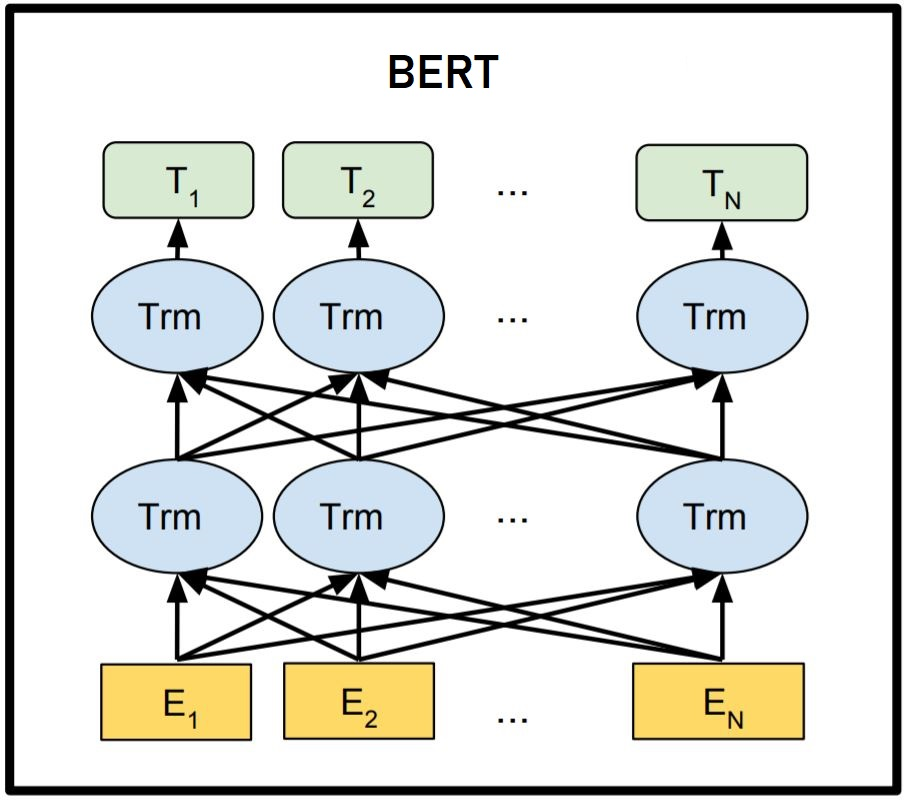
\includegraphics[width=12cm]{bert}}  
	\caption{BERT model architecture}
	\label{bertModel}
\end{figure}

	The model uses the encoder decoder pattern combined with a self-attention system to solve common natural language processing tasks.	Both the encoder and decoder consist of stacks of 6 hidden layers with similar architecture, separated in sub-layers. The encoder contains a multi-head attention sub-layer and a simple feed-forward layer. The two sub-layers are connected through residual connections followed by a layer normalization. The decoder works similar to the encoder with the addition of an second attention layers, which takes its input from the output of the encoder. 
	
	Transformers solve the parallelization incompatibility of current state-of-the-art systems on top of increasing the quality of the output. A transformer system reached a new single-model state-of-the-art BLEU score on the WMT 2014 English-to-German translation task, with a small cost of training compared to the previous best model.
	
\begin{figure}
\centerline{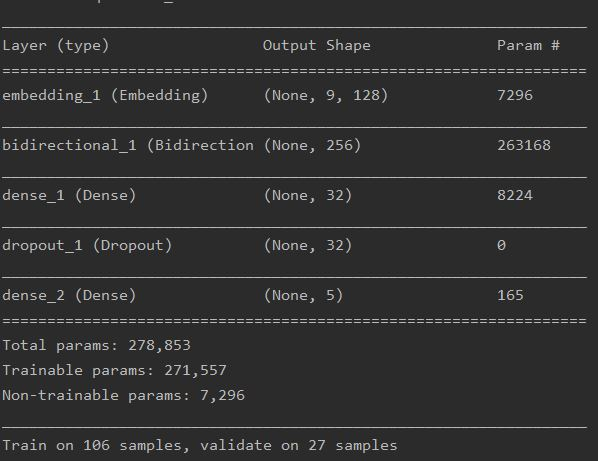
\includegraphics[width=12cm]{custmodel}}  
	\caption{Custom intent classifier model structure}
	\label{custmodel}
\end{figure}


\begin{figure}
\centerline{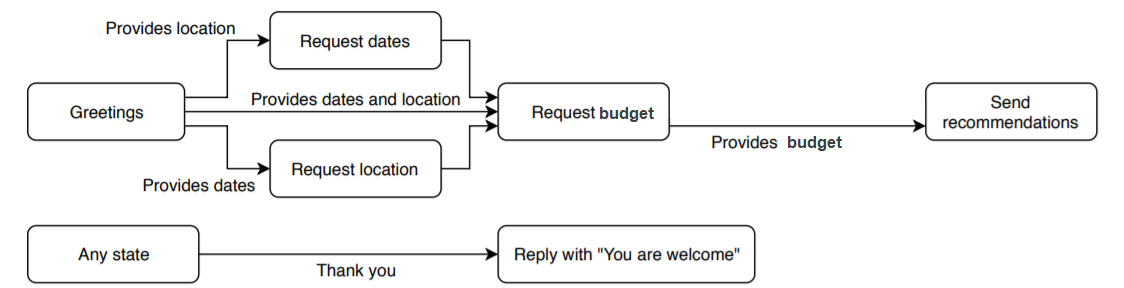
\includegraphics[width=\textwidth]{Img/statetrans.png}}  
	\caption{Diagram showing part of the state machine, with relevant transitions; this part is invoked when a user starts a new conversation with the bot}
	\label{statetrans}
\end{figure}


\begin{figure}
\centerline{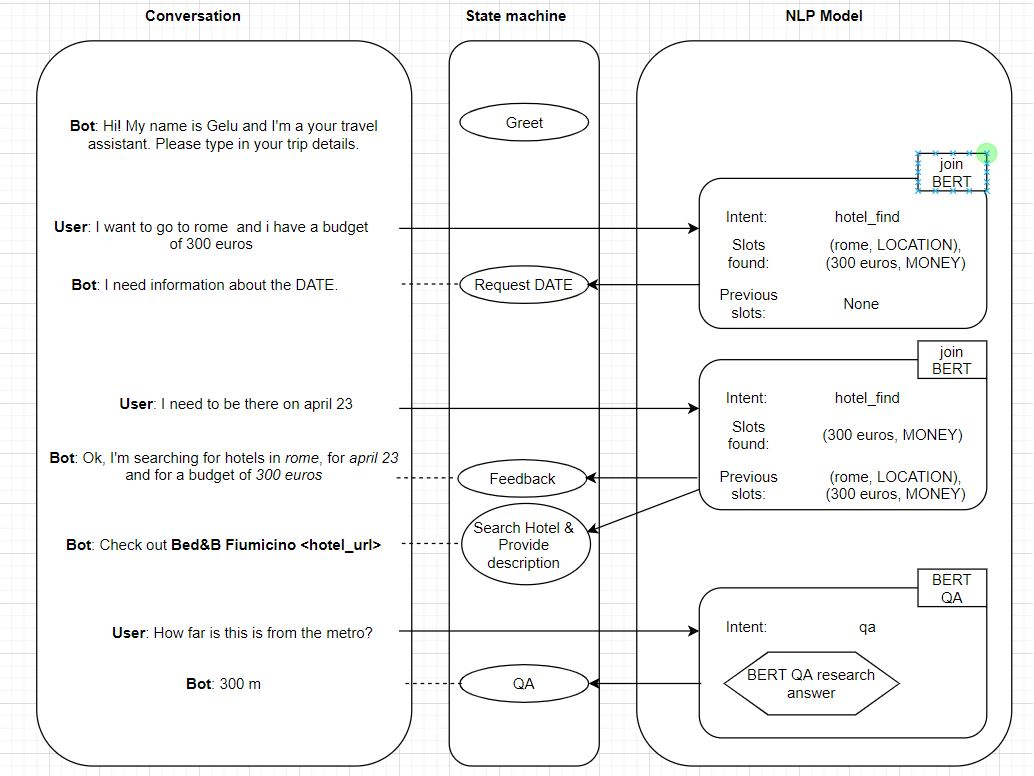
\includegraphics[width=\textwidth]{Img/stateM.JPG}}  
	\caption {Example of a conversation with our bot, with corresponding state transitions and model logic. First, the user message is processed by the intent model,
which classifies the message into one of several intents. Depending on the intent and current conversation state, the BERT QA model may need to be invoked. Then, a response is generated based on output of the models, and the conversation transitions to a different state.
}
	\label{stateM}
\end{figure}

BERT (Bidirectional Encoder Representations from Transformers) is a machine learning architecture, that presents state-of-the-art results on eleven natural language processing tasks \cite{bert}. BERT is a pretrained model which can then be optimized for downstream tasks. The implementation of downstream tasks can be done through fine-tunning or feature-based. Feature based approach implies architecture changes to accommodate for additional weight categories. The fine-tunnig approach, that BERT uses, adds an additional final layer to accommodate the weights for a specific set of data. The pretraining of the model is done in two steps: masked language model and next sentence prediction. MLM was needed because of the bidirectional nature and full connectivity of the model, without which nodes could find their word in the output of the previous nodes. Next sentence prediction proved to be very useful in natural language understanding tasks like question answering.

\subsection{Custom intent classification model}
\label{section:customModels}

The current model configuration of the intent classifier was achieved through experimentation. Although not being the best one obtained during the development phase, we had to simplify the model for performance reasons. 

The model architecture we settled to is composed of an embedding, a bi-directional and a dense layer with ReLu activation. We included dropout to avoid overfitting and a final dense layer with Softmax that produces the confidence values for each class. We can observe the network structure in Figure \ref{custmodel}.


\subsection{Chatbot module}
\label{section:chatbot}

The chatbot module is built as a state machine responsible of keeping track of the mandatory hotel features needed to perform the query over the hotels API. 

In the initial state of the bot, it is the first to initiate the conversation by greeting the user and encourage him/her to provide search criteria for the trip. 

Once the user responds, the intent of the message is computed, along with potential slots (features) contained. 
The features detected are persisted in memory and the conversation proceeds until all three key features are obtained. If the user does not provide the search parameters, the bot will request them successively. An example of this state transitions is provided in Figure \ref{statetrans}, and an example of a chatbot conversation, along with the internal states is provided in Figure \ref{stateM}.

When all the search criteria is filled in, the bot will fire a request to a hotel searching API, similar to Booking.com, that will retrieve the description of the hotel that best matched the search, sorted by the user rating. The relevance sorting was not addressed in this scope, but is a point of improvement for future work.

Having provided a the hotel suggestion, the user can address questions to the bot, and the answers will be looked up in the hotel description.


\section{Tools and technologies used}
\label{section:tools}

Among the frameworks and tools we used for the design and development of our system, we enlist the most important ones:
\begin{itemize}
	\item \textbf{Scikit-learn}: python machine learning library;
	\item \textbf{Pytorch}: open source machine learning library based on the Torch library, used for applications such as computer vision and natural language processing;
	\item \textbf{Tensorflow}: Pyhton library for building machine learning models;
	\item \textbf{Keras}:  Pyhton library that facilitates building neural networks;
	\item \textbf{SciPy}: a Python-based ecosystem of open-source software for mathematics, science, and engineering that has a very mature NLP module;
	\item \textbf{React}: Javascript framework used for developing our user interface;
	\item \textbf{Electron}: allows for the development of desktop GUI applications using web technologies. We used it to be able to run our chatbot both as a web and desktop application;
	\item \textbf{Matplotlib}: provides an object-oriented API for embedding plots into applications using general-purpose GUI toolkits
	\item \textbf{Flask}: web framework for building APIs in Python
\end{itemize}

\section{Feature definition and extraction}
\label{section:features}

We defined five intent classes as follows: 
\begin{itemize}
	\item greet
	\item thank
	\item hotel\_find
	\item stop
	\item assist.
\end{itemize}

The hotel\_find intent can contain a set of 19 features, as listed in Figure \ref{slots}.

\begin{figure}
\centerline{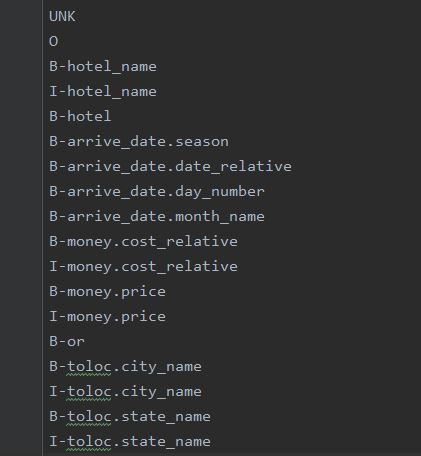
\includegraphics[width=10cm]{slots}}  
	\caption{Slot classification features}
	\label{slots}
\end{figure}

Each sentence produced by the user is analyzed from the intent point of view and slots contained. Each prediction retrieves the intent detected and a dictionary containing the pairs of slot names and slot values found inside the phrase, if any.

\section{Improvements and optimisations}
\label{section:optim}

The first version of the application had a very big response-time for the predictions and API calls. We performed a memory footprint reduction task, aiming to decrease resource utilization of both the models and of the state machine, by reducing variable and object allocation and decreasing the network depth. Response time improvements: 

        3.8 seconds avg. -> 1.1 seconds avg. 
        
        (request completion-time measured in Chrome dev tools).



\chapter{Application (numerical validation)}
\label{chapter:applicaion}

We present in this chapter the results obtained on the custom intent classifier and as well as on the BERT-based model (joined intent and slot filling), and a comparison with state-of-the-art results.

\section{Methodology}
\label{section:methodology}

\begin{itemize}
	\item As our intent classification and slot filling tasks are essentially classification problems, for evaluation we use precision, recall and F1 scores, together with validation loss. For the question answering task we measure the F1 score and the exact matches percentage.
	\item We aim to get better insight on the advantages of BERT versus a simple classifier in the context of intent classification, as well as to test its performance on smaller and real world data.
\end{itemize}


\section{Data}
\label{section:data}

As mentioned in the previous section, we performed transfer-learning and fine-tuning on pre-trained BERT models, that were evaluated on state-of-the-art datasets. For the intent classification and slot filling task, we used a pre-trained model and trained it on the ATIS \cite{gok10} and Snips \cite{ali16} datasets. For the question answering task we used a pre-trained BERT model on SQuAD 2.0 []. We then performed transfer-learning and trained these models on custom data sets that we created.

The dataset was one of our main issues since we did not find an open-source one that satisfied our requirements. We managed to gather a sample on 100 data entries and to model them for our training and evaluation tasks, but this small amount of training data was one of the reasons why our model did not reach better accuracy.

\subsection{Data preparation}
\label{section:dataprep}

When dealing with natural language, data can be very complex and unorganised. As such, simplifying as best as possible the dataset is an essential endeavour in order to reach good accuracy. For both our intent classification and slot filling tasks, we applied a series of data pre-processing techniques.


\begin{itemize}
	\item \textbf{data cleaning}: the raw data obtained from the future user needs to be cleared of all the factors that could create noise. As such, we eliminated punctuation and special characters and tokenized the sentences into words. We then lowercased all words;
	\item \textbf{lemmatization}: this process ensures that the words are more valuable and more easily recognisable, by removing any trace of inflections from a word. An example of such a process is the transformation of plural forms into singular.
	\item \textbf{data splitting}: we divided out data into training (80\%) and evaluation (20\%) sets, to obtain actual results of how the model performs on unfamiliar data.
	\item \textbf{data integration}: in our joined BERT approach, we composed an extensive dataset combining both information about the intents and information about the slots that need to be filled in each phrase.
\end{itemize}
 

\section{Results}
\label{section:results}

Comparing the results obtained by our two approaches, the custom intent classifier with SpaCy slot filling, and the joined BERT we observe that while our custom intent classifier did perform better on intent classification alone, it obtained poorer results when integrated with the slot filling agent.

\begin{figure}
\centerline{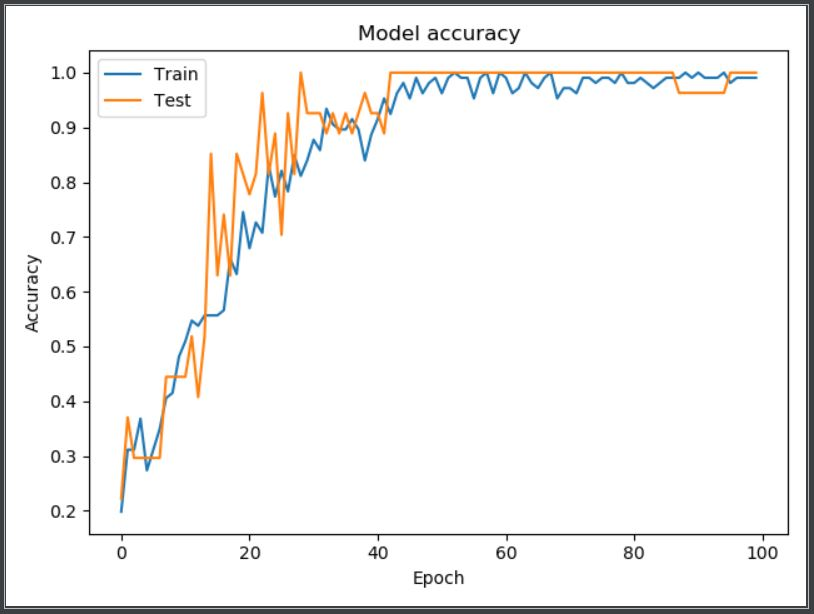
\includegraphics[width=12cm]{Img/m1acc.JPG}}  
	\caption{Custom intent classifier accuracy after 100 epochs}
	\label{accM1}
\end{figure}

We defined four intent classes for our custom intent classifier. The results obtained after 100 epoch are presented in Figures \ref{accM1} and \ref{lossM1}.

\begin{figure}
\centerline{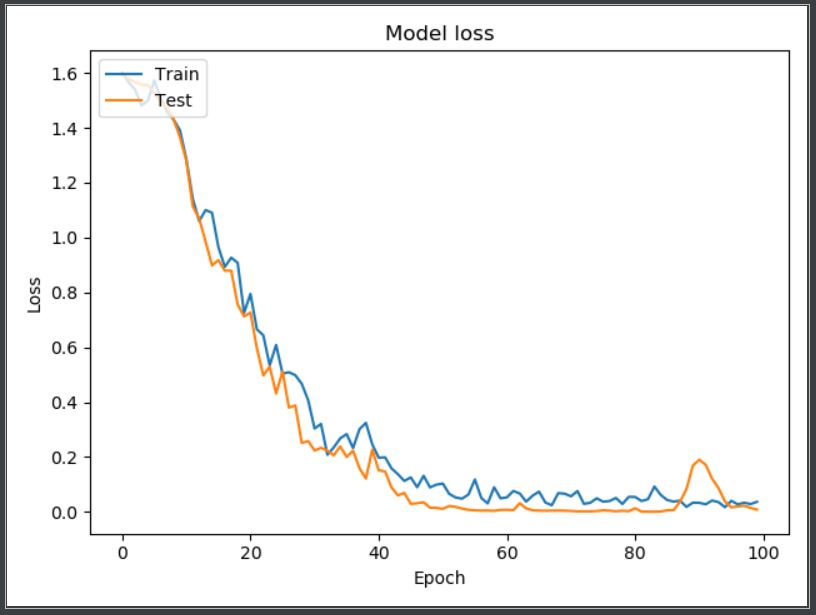
\includegraphics[width=12cm]{Img/m1loss.JPG}}  
	\caption{Custom intent classifier validation loss after 100 epochs}
	\label{lossM1}
\end{figure}

We obtained an accuracy of 97\% for the custom intent classifier and of 92.59\% for the Joined BERT model. The BERT model behaved better in a real-life usage simulation of the application.

\section{Back-end Python application}
\label{section:BE}

The back-end application comprehends both the AI modules, the chatbot itself (state-machine) and the Web API written in Flask. We illustrate the main architecture and relations between the application models below.

\begin{figure}
\centerline{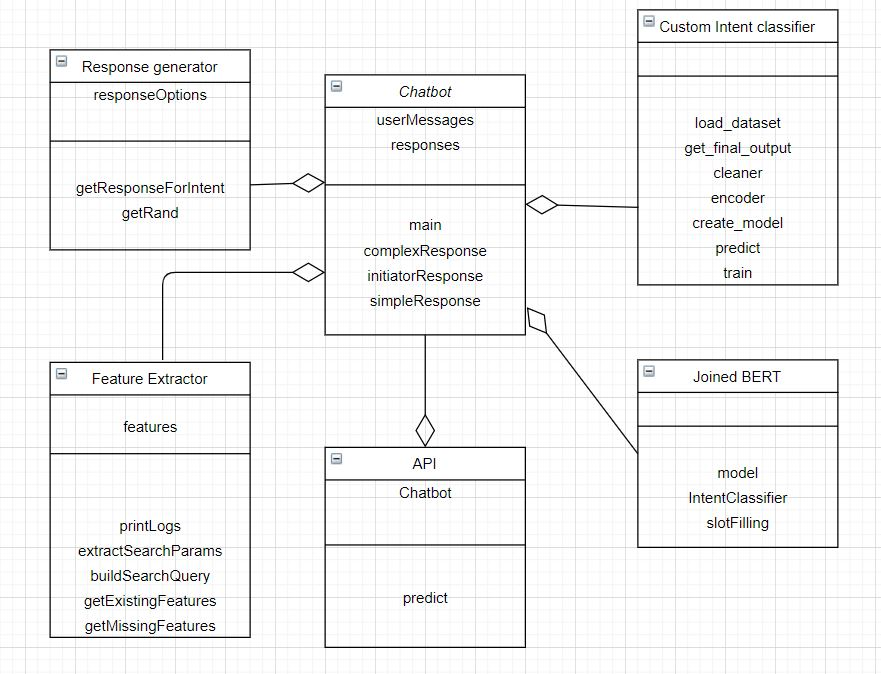
\includegraphics[width=\linewidth]{Img/archDiagr.JPG}}  
	\caption{The Back-end application architecture}
	\label{beArch}
\end{figure}


\section{User interface}
\label{section:UI}

As far as our user interface is concerned, we created a Front-End application that connects to our Back-End in python. The application was written in React and encapsulated in the Electron framework in order for it to be used as both a web and desktop application. 

The interface is a simplistic one, as we believe minimalism is an important factor towards user friendliness. It presents a chat window with an input box and a button for sending the messages. Animations are available for when the chatbot is processing ("thinking") the response, and the window is scrolled automatically when new messages (that would exceed the viewport) are added.

\begin{figure}[ht!]
\centerline{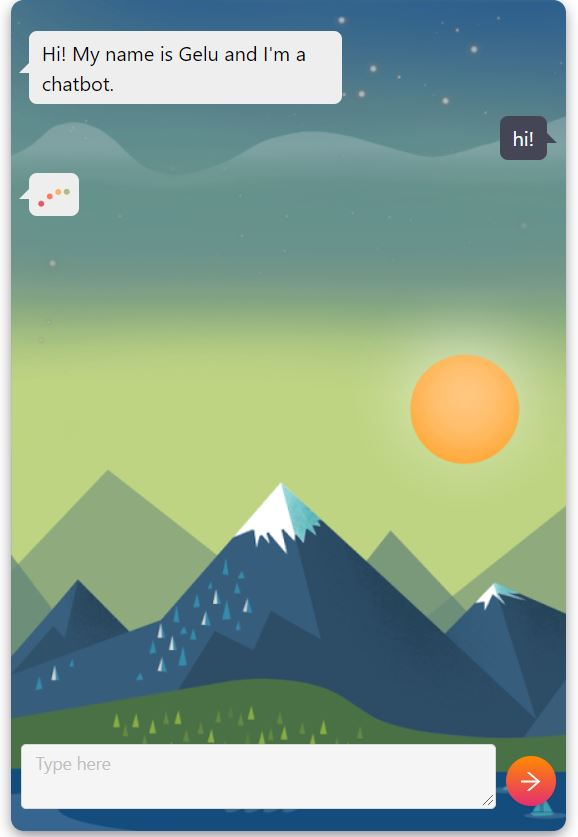
\includegraphics[width=12cm]{Img/uiscreen.JPG}}  
	\caption{The application user interface}
	\label{uiscreen}
\end{figure}


\section{Discussion}
\label{section:discussion}

Our two approaches, the custom intent classifier with SpaCy slot filling, and the joined BERT presented in \ref{section:algorithmDescription}, have unraveled interesting findings. While our custom intent classifier did perform better on intent classification alone, it obtained poorer results when combined with the slot filling task. Correlating the two datasets into one, that was fed to the joined BERT model has reached the best accuracy, being able to make more insightful connections between the intent and the slots. 

We did not reach state of the art results, mostly due to our lack of data. We would like to employ more time to extend the datasets as well as adding more intents and slots to see how well the two models scale.


\chapter{Conclusion and future work}
\label{chapter:concl}

In this paper we have demonstrated the applications of the BERT model for solving several NLP tasks: intent classification, slot filling and question answering. 

We analyzed a custom built classifier using a bi-LSTM model against the BERT based implementations and connected them through a state-machine application with another intelligent agent able to perform question answering on the result obtained from the first model. Results were positive for both models, but did not reach state-of-the-art accuracy. 

Furthermore, one of the goals we intended to achieve through this paper was to demonstrate the use of such models in a real-world application context, namely by building a task-oriented chatbot that helps users find accommodations for their vacations. The proof of concept illustrated within this research demonstrates that an intelligent assistant can be successfully used for a practical use case and is fairly user-friendly.

One of the shortcomings that impacted our results was the lack of a comprehensive hotels dataset, such that we had to create our own dataset and have a limited volume of training data.

As future work, we would like to improve the accuracy of the current model, by gaining more insightful data. Moreover, adding new intents and slots for other key-features relative to the booking domain would increase the user-friendliness, operability and usefulness of the assistant. Adding more intents would also support more complex dialog flows and provide a more authentic conversation experience.

Another feature that could be added to our system is the capability of the bot to understand when there is the need to request assistance from a specialised operator (human). Then the bot could send the history of the conversation to the operator that will take over the conversation. This feature could be somewhat facilitated by the fact that our system already preserves the chat history locally. 

Last but not least, we propose an integration with chatbot smart devices like Amazon Echo (Alexa) that could combine both written and spoken (voice) input.


\bibliographystyle{plain}
\bibliography{BibAll}


\end{document}

